\section{Arsitektur Sistem}
Sistem yang akan dikembangkan mengguanakan arsitektur RESTful untuk berkomunikasi antara \emph{client} dengan server. RESTful dipilih dengan tujuan agar mudah untuk mengembangkan \emph{client} berbasis multi-platform. Server menerima \emph{request} pertanyaan dalam format text/plain ataupun text/json, kemudian respon diberikan dalam format ojek json atau xml.

Masing-masing ontologi diletakkan di lokasi yang berbeda dan dapat diakses secara terpisah melalui protokol HTTP sehingga akan lebih mudah diakses baik oleh aplikasi yang dikembangkan ini sendiri, maupun aplikasi lain yang nantinya ingin memanfaatkan ontologi yang telah dibangun. Arsitektur sistem yang dikembangkan dalam penelitian ini ditunjukkan dalam gambar \ref{fig:arsitektur_sistem}

\begin{figure}[ht]
    \centering
    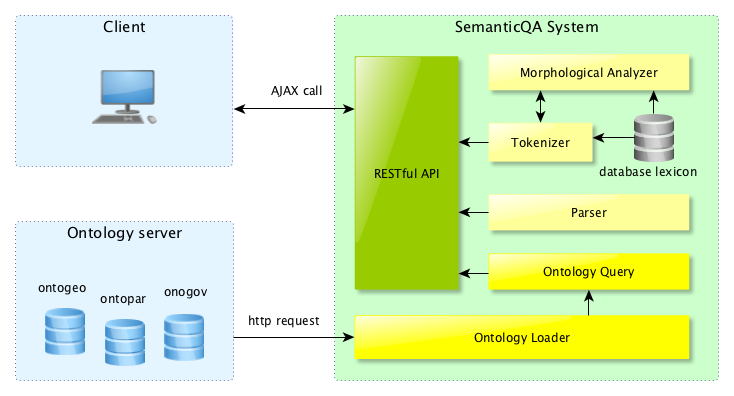
\includegraphics[width=1\textwidth]{arsitektur_sistem}
    \caption{Arsitektur sistem yang akan dikembangkan}
    \label{fig:arsitektur_sistem}
\end{figure}